% ============================================================
%  Section 1 — gentle intro to the "five integers, sum mod 3" puzzle
%  Designed to drop into an article-class document.
%  Required packages (add to preamble if not already present):
%     \usepackage{amsmath, amssymb}
%     \usepackage{graphicx}
%     \usepackage{svg}          % only if including the SVG directly
%     % --- alternatively, pre-convert the SVG to PDF and use \includegraphics ---
% ============================================================

\section{The picture, in plain words}
\label{sec:intro}

Suppose I hand you five whole numbers --- any five, chosen however you
like. I now claim that hiding somewhere inside your five numbers, there
are three whose sum is divisible by $3$. Always. No exceptions, no
clever counter-example.

That's a strange-sounding claim, so let's slow down and build the
picture before we try to prove it.

\paragraph{Three buckets.}
Every integer, no matter how large or how negative, leaves one of three
possible remainders when you divide it by $3$: either $0$, $1$, or $2$.
So we can sort the integers into three buckets by remainder --- this is
the top row of Figure~\ref{fig:buckets-and-triples}. The number $6$
lands in bucket $0$; $7$ lands in bucket $1$; $8$ in bucket $2$; $9$
back in bucket $0$; and so on. The bucket is the only thing about a
number that matters here --- once we're hunting for sums divisible by
$3$, we can forget the number itself and just remember which bucket it
came from.

\paragraph{What does it take to win?}
Now ask a smaller question: if I pick three bucket labels --- and I'm
allowed to pick the same bucket more than once --- which combinations
of labels add up to a multiple of $3$?

There are surprisingly few. They're shown in the bottom row of
Figure~\ref{fig:buckets-and-triples}:
\begin{align*}
  0 + 0 + 0 &= 0 \quad\checkmark \\
  1 + 1 + 1 &= 3 \quad\checkmark \\
  2 + 2 + 2 &= 6 \quad\checkmark \\
  0 + 1 + 2 &= 3 \quad\checkmark
\end{align*}
That's it. Four winning triples, and no others. Every other combination
of three labels --- say $0+0+1$, or $1+1+2$ --- leaves a stubborn
non-zero remainder behind.

Notice the shape of the winners: either all three labels are
\emph{the same}, or all three labels are \emph{all different}. There is
no middle ground. That's the lever we're going to pull.

% ----- Figure -----
\begin{figure}[h]
  \centering
  % Option A: include the SVG directly (requires the `svg` package + Inkscape)
  % \includesvg[width=0.85\textwidth]{mod_3_buckets_and_winning_triples}
  %
  % Option B (recommended for portability): convert the SVG to PDF first, then:
  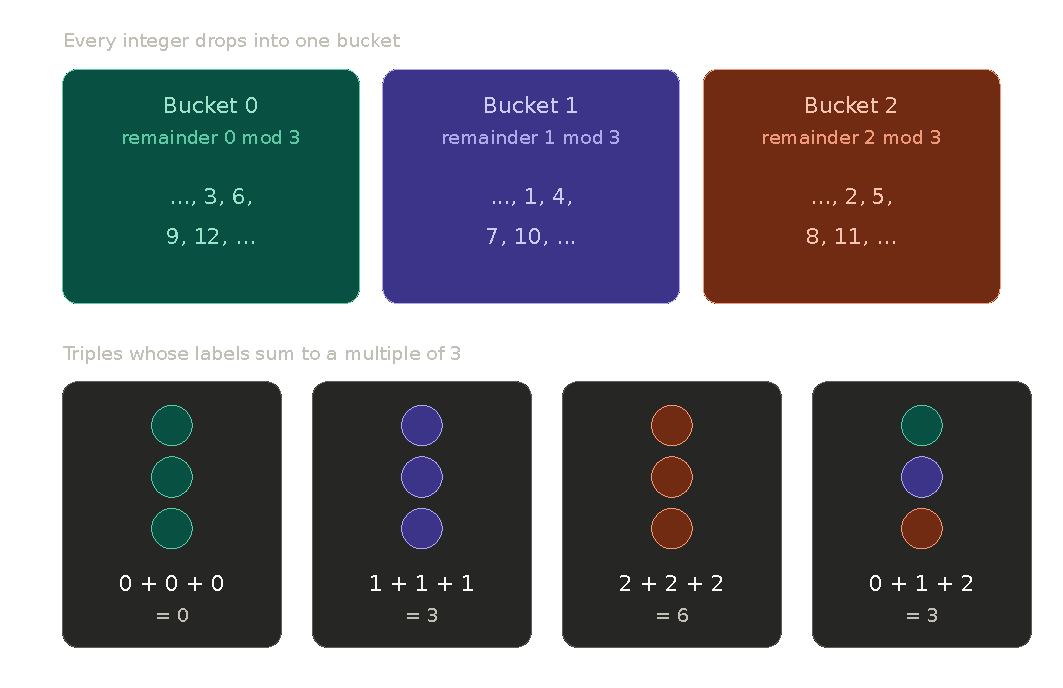
\includegraphics[width=0.85\textwidth]{mod_3_buckets_and_winning_triples}
  \caption{\textbf{Top:} every integer lives in one of three buckets,
    determined by its remainder mod~$3$.
    \textbf{Bottom:} the only four ways to choose three bucket-labels
    (with repetition) whose sum is a multiple of~$3$. Either all three
    come from the same bucket, or one from each.}
  \label{fig:buckets-and-triples}
\end{figure}

\paragraph{The puzzle, restated.}
We started with \emph{``given any five integers, must there be three of
them whose sum is divisible by $3$?''} Once our five integers are
sorted into the three buckets, the question collapses into something
much friendlier:

\begin{quote}
  If I drop $5$ balls into $3$ buckets, can I always find either\\
  \textbf{(a)} three balls in a single bucket, or\\
  \textbf{(b)} at least one ball in every bucket?
\end{quote}

Because (a) is ``all three labels the same'' and (b) is ``all three
labels different'' --- and those are exactly the winning
configurations.

So the original problem about sums divisible by $3$ is now a much more
visual question about balls and buckets. Before reading on, give it a
moment: with only $5$ balls and only $3$ buckets, can you picture any
arrangement that dodges \emph{both} (a) and (b)?

\paragraph{A peek at the intuition.}
It feels like the balls are forced to do one of two things --- either
they \emph{cluster} (some bucket gets crowded, $\geq 3$) or they
\emph{spread} (every bucket gets at least one). What we'll argue in the
next section is that there is no way to thread the needle between
these two outcomes, and that both outcomes happen to be wins. The
engine driving this is the pigeonhole principle, and once it's spelled
out properly the whole thing fits on half a page.

After the proof we'll come back to the natural follow-up: is $5$ the
smallest number that works, or could we have managed it with $4$? That
question turns out to open onto a much larger landscape --- and
exploring that landscape is what the rest of this paper is for.
